\chapter{Analyse}
In diesem Kapitel werden die in Kapitel 4 vorgestellten Systeme analysiert.

\section{128MB Konfigurationen}
Zunächst werden alle Tests gegen die 128MB Konfigurationen ausgeführt. In den folgenden Sektionen wird dann die Speicher- und Prozessorgröße erhöht. 

\subsection{Pipe-Clean Tests}
Zunächst wird die Performance der SUTs in der bestmöglichen Situation mit einem einzigen Nutzer ermittelt. Ziel dessen ist es, eine Vergleichsgrundlage für die darauf folgenden Tests zu schaffen. Der Test wurde mit einer Dauer von zehn Minuten mit einem aktiven Benutzer für jeden Use-Case durchgeführt. Jeder Test wurde drei mal ausgeführt und die Metriken über die Gesamtmenge der Daten aggregiert. Bei den Requests wurde die Summe gebildet, bei den durchschnittlichen Requests pro Sekunde das arithmetische Mittel.

\begin{figure}[H]
    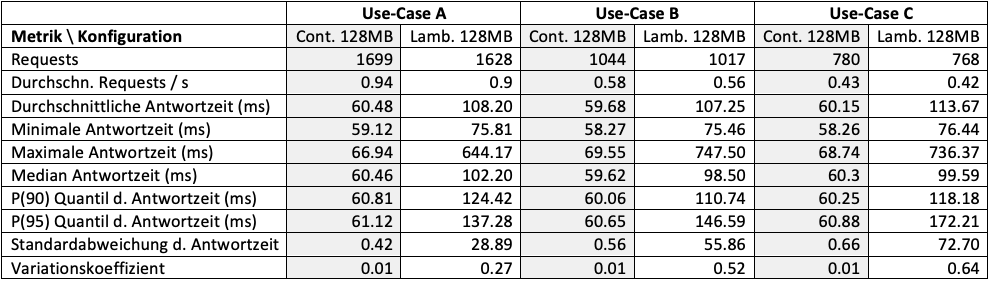
\includegraphics[width=\textwidth]{img/pipe128-comparison.png}
    \caption[Vergleich der Pipe-Clean Tests für 128MB]{Vergleich der Pipe-Clean Tests für 128MB}
    \label{fig:pipe128-comparison}
\end{figure}

Abbildung \ref{fig:pipe128-comparison} zeigt die Ergebnisse des Tests für die Funktionen mit 128MB CPU bzw. RAM. Es ist zu erkennen, dass die Container Anwendung in allen Fällen eine deutlich geringere Antwortzeit als die Lambda Anwendung aufweist. Im Median ist der Container bei Use-Case A etwa 41,74ms schneller als die Lambda-Funktion. Während die maximale Antwortzeit bei ersterer nur etwa 10,7\% über dem Median liegt, ist sie bei der Lambda-Funktion etwa 630\% über ihrem Median. Dass die Lambda-Anwendung eine überaus große Varianz in ihren Antwortzeiten aufweist, wird auch in ihrer Standardabweichung von bis zu 72ms deutlich, währende sie bei der Container Anwendung in allen drei Use-Cases unter 1ms liegt. Interessanterweise liegt die Antwortzeit der Lambda-Anwendung im Median in allen drei Use-Cases bei ähnlichen Werten um ca. 100ms. Andererseits nimmt die Standardabweichung und das P(95) Quantil der Antwortzeit bei Use-Case B im Vergleich zu Use-Case A deutlich zu. Und auch bei Use-Case C ist ein deutlicher Anstieg der Werte zu beobachten. Vermutlich ist dies auf die größere Anzahl an angefragten Endpunkten zurückzuführen, da dadurch mehr Coldstarts durchgeführt werden müssen. Auch bei der Container-Anwendung ist keine Veränderung der Median-Antwortzeit um ca. 60ms festzustellen. Die Standardabweichung der Antwortzeit erhöhte sich nur leicht von 0,42 auf 0,66.

Anhand der Vergleichstabelle lassen sich auch Erkenntnisse über die einzelnen Use-Cases ableiten. Use-Case A setzt sowohl bei der Container- als auch bei der Lambda-Anwendung deutlich mehr Requests in der Sekunde ab als es bei den Use-Cases B und C der Fall ist. Dies liegt an der größeren Think-Time, wie sie bei den Use-Cases mit Benutzer-Eingaben zum Einsatz kommt.

\subsection{Stress-Tests}
Um RQ1 zu beantworten, muss zunächst die maximale Auslastung eines einzelnen Containers ermittelt werden. Dazu wurden mehrere Stress-Tests durchgeführt. Ein Stress-Test dient dazu, die Grenzen des SUTs herauszufinden. Da Lambda ein von Natur aus automatisch horizontal skalierendes System ist, werden die Test zunächst für die Container-Anwendung durchgeführt und im Anschluss die Lambda-Anwendung mit der gleichen Test-Konfiguration getestet. Dadurch kann das Verhalten der Funktionen bei langsamem Anstieg der Benutzer evaluiert werden. Die Anzahl der VUs wird bei den Stress-Tests wie von Molyneaux\cite{molyneaux_art_2014} empfohlen immer stufenweise erhöht. Das bedeutet, dass nach jedem Ramp-Up (ein linearer Anstieg) eine gleichlange Periode mit einer konstanten Anzahl an Benutzern folgt. Abbildung \ref{fig:stress-vus-example} verdeutlicht dies anhand eines Stress-Tests, bei dem bis zu 600 gleichzeitige Virtuelle Benutzer erstellt werden. In 60 Sekunden Zeitabschnitten werden nach und nach immer 60 Benutzer hinzugefügt. Daraufhin folgt eine weitere 60 Sekunden lange Periode, in der die Anzahl der VUs nicht weiter erhöht wird. Der gesamte Test hat demnach eine Dauer von 40 Minuten. Eine Cooldown-Phase nach den vollen 600 Benutzern wird hier nicht eingelegt, da das Skalierungsverhalten nicht untersucht wird.

\begin{figure}[H]
    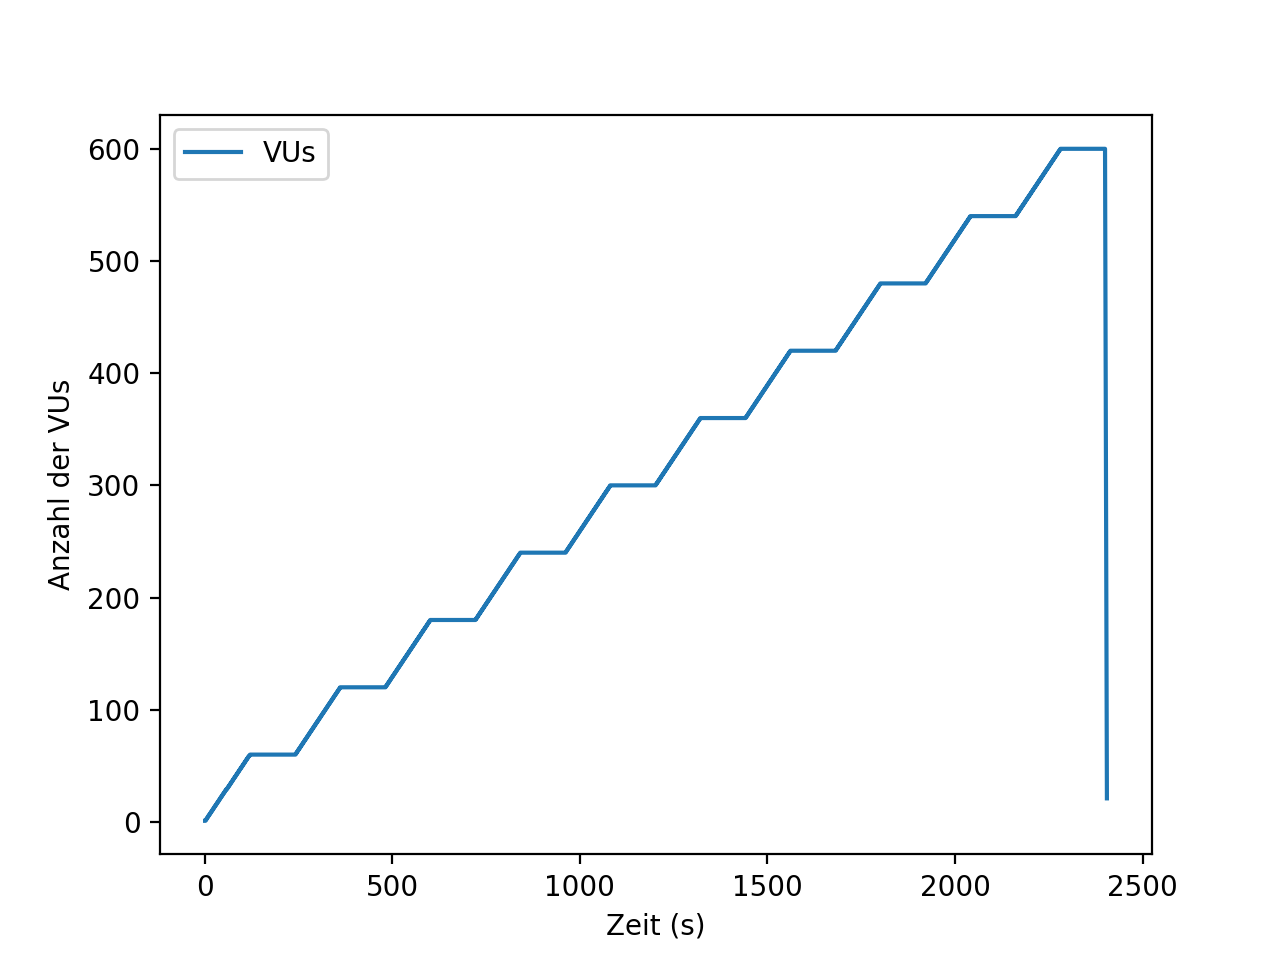
\includegraphics[width=\textwidth]{img/stress-vus-example.png}
    \caption[Beispiel-Anstieg der gleichzeitigen VUs für einen Stress Test]{Beispiel-Anstieg der gleichzeitigen VUs für einen Stress Test}
    \label{fig:stress-vus-example}
\end{figure}

\subsubsection{Container}
Für die containerisierte Anwendung in der 128MB Konfiguration wurden mehrere Stress-Tests durchgeführt, bis das Limit der gleichzeitigen Benutzer identifiziert werden konnte. Abbildung \ref{fig:fargate128-stress-comparison} zeigt die getesteten Use-Cases und die Stress-Test Konfiguration. 

\begin{figure}[H]
    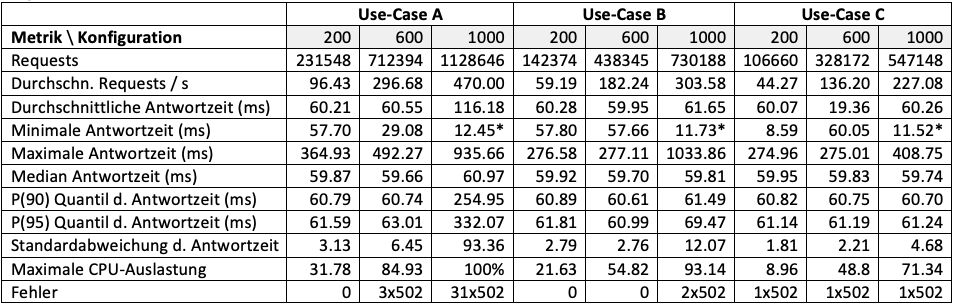
\includegraphics[width=\textwidth]{img/fargate128-stress-comparison.png}
    \caption[Fargate 128MB Stress-Test Vergleich]{Fargate 128MB Stress-Test Vergleich}
    \label{fig:fargate128-stress-comparison}
\end{figure}

Der erste Test wurde mit bis zu 200 Benutzern durchgeführt. Dabei konnte jedoch nur bis zu 32\% der CPU-Auslastung des Container-Clusters erreicht werden; In Use-Case B waren es sogar nur fast 22\%. Der geringen Auslastung entsprechend, war kaum eine Veränderung der Antwortzeiten gegenüber den Pipe-Clean Tests festzustellen (vgl. mit Abbildung \ref{fig:pipe128-comparison}). Einige Metriken lagen sogar unter den Grundwerten. Lediglich die maximale Antwortzeit hat sich bei allen Use-Cases, bspw. bei Use-Case A von 60,46ms auf 364,93ms, deutlich erhöht. Dies ist allerdings nur vereinzelt der Fall, da immer noch 95\% aller Anfragen innerhalb von ca. 62ms beantwortet werden und auch an der Standardabweichung hat sich nicht großartig verändert. 

Bei dem zweiten Stress-Test mit bis zu 600 VUs, änderte sich nicht viel im Vergleich zu dem Test mit 200 Benutzern. Es konnten zwar bis zu 84,93 Prozent CPU-Auslastung erreicht werden und die maximale Antwortzeit stieg erneut an, auf fast 500ms. Trotz dessen konnten von dem einzelnen Container 95\% der Anfragen innerhalb von knapp 63ms beantwortet werden. Problematisch zeigten sich hier drei Requests, die vom Server nicht mehr beantwortet werden konnten und den 502 Fehlercode zurücksendeten. Dies entspricht jedoch nur 0,00042\% aller in diesem Stress-Test durchgeführten Requests.

\begin{figure}[H]
    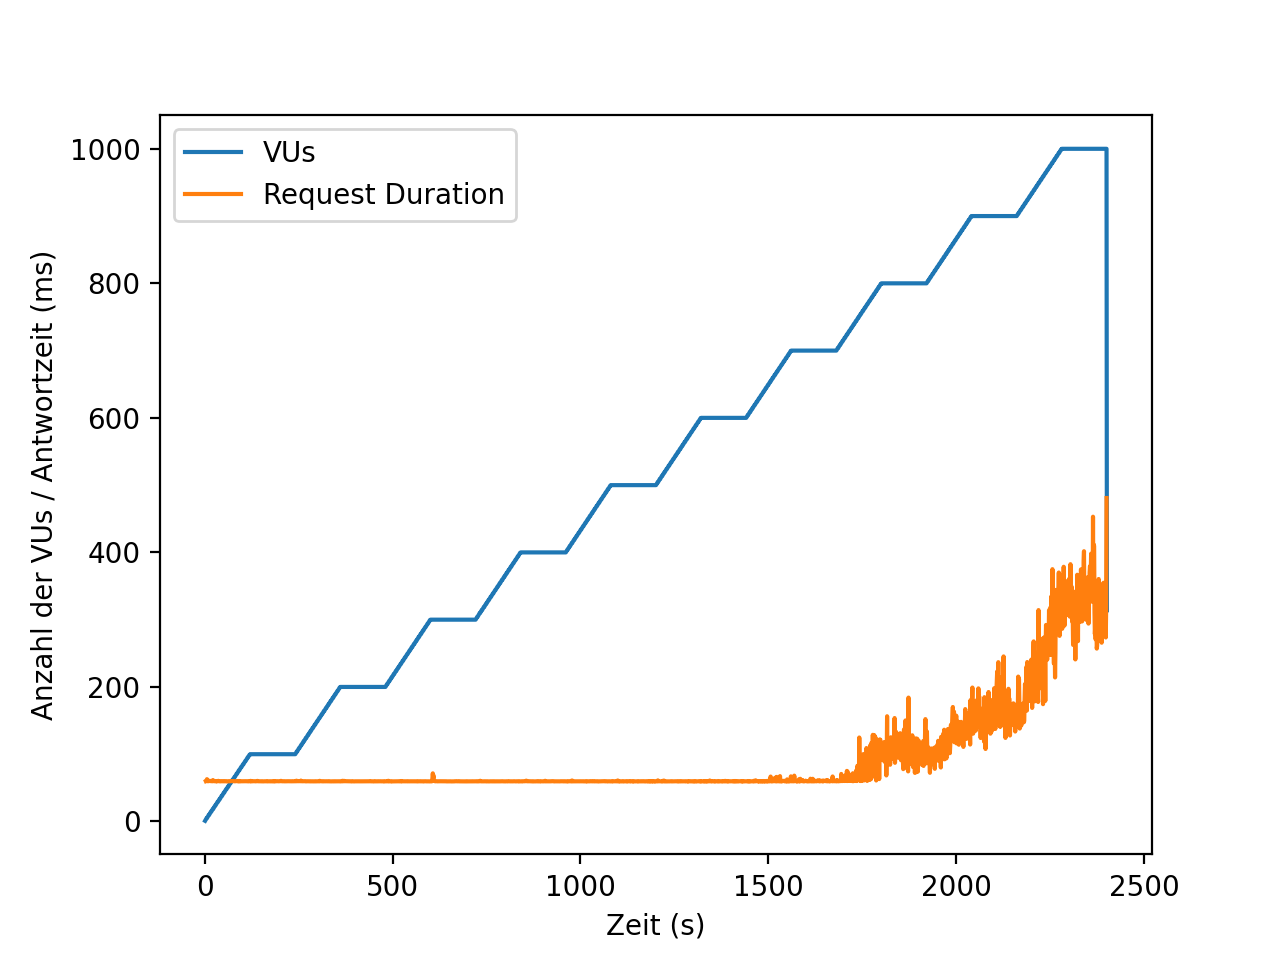
\includegraphics[width=\textwidth]{img/fargate128-stress1000.png}
    \caption[Container Stress-Test 1000VUs]{128MB Container Stress-Test 1000VUs Use-Case A}
    \label{fig:fargate128-stress1000}
\end{figure}

Der dritte Stress-Test für den 128MB Container wurde mit bis zu 1000 VUs durchgeführt. Abbildung \ref{fig:fargate128-stress1000} zeigt den zeitlichen Verlauf dieses Tests für Use-Case A. Es wird dabei die Anzahl der virtuellen Benutzer und die Antwortzeit im Median pro Sekunde dargestellt. Es wird deutlich, dass die Antwortzeit ab ca. 700 VUs deutlich ansteigt. Dies deckt sich der von AWS Cloudwatch gemessenen CPU-Auslastung von knapp unter 100\% die bei dieser Nutzerzahl gemessen wurde. In den Perioden mit konstanten Nutzerzahlen können die Requests besser verarbeitet werden und die Kurve geht wieder leicht herunter. Während des Tests wurden trotz einer CPU-Auslastung von teilweise 100\% nur 31 HTTP 502 Fehlercodes vom Server ausgelöst, was einer Quote von 0,0027\% entspricht. Die Antwortzeit konnte im Median weiterhin bei etwa 60ms gehalten werden; die durchschnittliche Antwortzeit stieg mit 116,8ms auf fast das doppelte des Grundwertes an.  
Bei Use-Case B lag die erreichte Prozessor-Auslastung bei 93,14\%. So wurden keine deutlichen Abweichungen ausgelöst. Die Standardabweichung stieg leicht an, liegt aber immer noch deutlich unter dem Wert des Pipe-Clean Tests der 128MB Lambda Funktion.

\subsubsection{Lambda}
Nachdem die maximale Performance des 128MB Containers ermittelt wurde, werden im Anschluss die gleichen Stress-Tests für die Lambda-Anwendung mit 128MB durchgeführt. Abbildung \ref{fig:lambda128-stress-comparison} zeigt die Ergebnisse. Für Use-Case A lässt sich erkennen, dass die Standardabweichung bei 200 und 600 VUs noch um die 19 beträgt, während bei 1000 Usern auf fast 55 ansteigt. Dies könnte allerdings an den extrem langen maximalen Antwortzeiten von bis zu 29.037ms liegen, die durch die Fehler verursacht werden. Die großen Fehler-Latenzen stehen im Gegensatz zu der Container Anwendung, bei der die maximale Antwortzeit immer noch knapp unter einer Sekunde lag. Auffallend ist, dass Fehler mit HTTP Statuscode 500 etwa 10s Antwortzeit aufweisen, während Fehler mit HTTP Statuscode 504 die fast 30s lange Latenz erzeugen. Die bei der Container-Anwendung erzeugten HTTP 502 Fehlercodes, führen stattdessen zu  Antwortzeiten von 12ms - 260ms. 

\begin{figure}[H]
    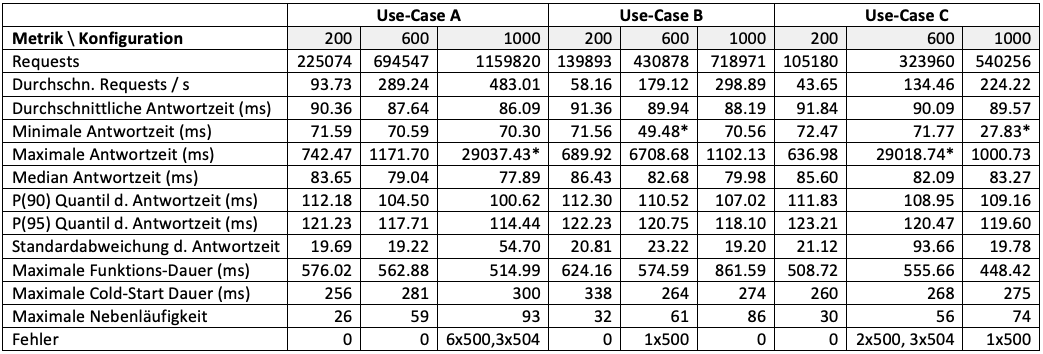
\includegraphics[width=\textwidth]{img/lambda128-stress-comparison.png}
    \caption[Lambda 128MB Stress-Test Vergleich]{Lambda 128MB Stress-Test Vergleich}
    \label{fig:lambda128-stress-comparison}
\end{figure}

Bei der Durchführung der Stress-Tests für die 128MB Lambda-Anwendung fällt außerdem auf, dass die Antwortzeit im Median bei steigenden Nutzerzahlen zu sinken scheint. Bei bis zu 200 VUs lag sie für Use-Case A noch bei 83.65ms, während sie bei bis zu 1000 VUs auf 77.89ms sank. Die Werte für Use-Case B scheinen einem ähnlichen Prinzip zu unterliegen. Es ist jedoch aktuell nicht bekannt, warum dies der Fall ist. Vermutlich provisioniert AWS die Funktionen schneller je mehr Anfragen sie erhalten. Trotz dessen, liegt die Antwortzeit im Median immer noch deutlich über der des 128MB Containers; die Differenz ist allerdings im Vergleich zu den Pipe-Clean Tests von 41,74ms auf 16.92ms gesunken (Use-Case A).

Zwischen den Use-Cases wird ebenfalls ein Unterschied in der Anzahl der nebenläufigen (concurrent) Lambda-Funktionen deutlich. Während bei 200 und 600 VUs für Use-Case B noch mehr Funktionen bereitgestellt wurden als für Use-Case A, zeigt sich für 1000 VUs ein umgekehrtes Bild. In diesem Fall, übertrifft der erste Use-Case den zweiten um 7 nebenläufige Funktionen. Dies ist interessant gegenüber RQ5, da es der Hypothese widerspricht, dass bei einer einzelnen angefragten Funktion weniger Coldstarts durchgeführt werden müssen als bei mehreren Funktionen (H5). Grund dafür ist vermutlich jedoch die geringere Anzahl der Requests pro Sekunde bei Use-Case B. 

\subsection{Load-Tests}
Für RQ2 soll die Performance unter normalen Nutzerzahlen mit der von schnell ansteigenden Nutzerzahlen verglichen werde. Dazu wird zunächst ein Load-Test für die in den vorangegangenen Stress-Tests ermittelten Nutzer-Grenzen der Container-Anwendung durchgeführt. Im Anschluss wird ein Spike-Test mit der gleichen Benutzerzahl durchgeführt. Ziel dessen ist es, die Performance der Anwendungen unter rasch ansteigender Last zu ermitteln. 

In den bisherigen Stress-Tests wurden nur langsame Anstiege (Ramp-Ups) durchgeführt. Für den Container wurde eine maximale Belastbarkeit von ca. 700 Benutzern ermittelt. Deshalb wird nun für den Load-Test von einem normalem Load von 600 Benutzern ausgegangen. 

\begin{figure}[H]
    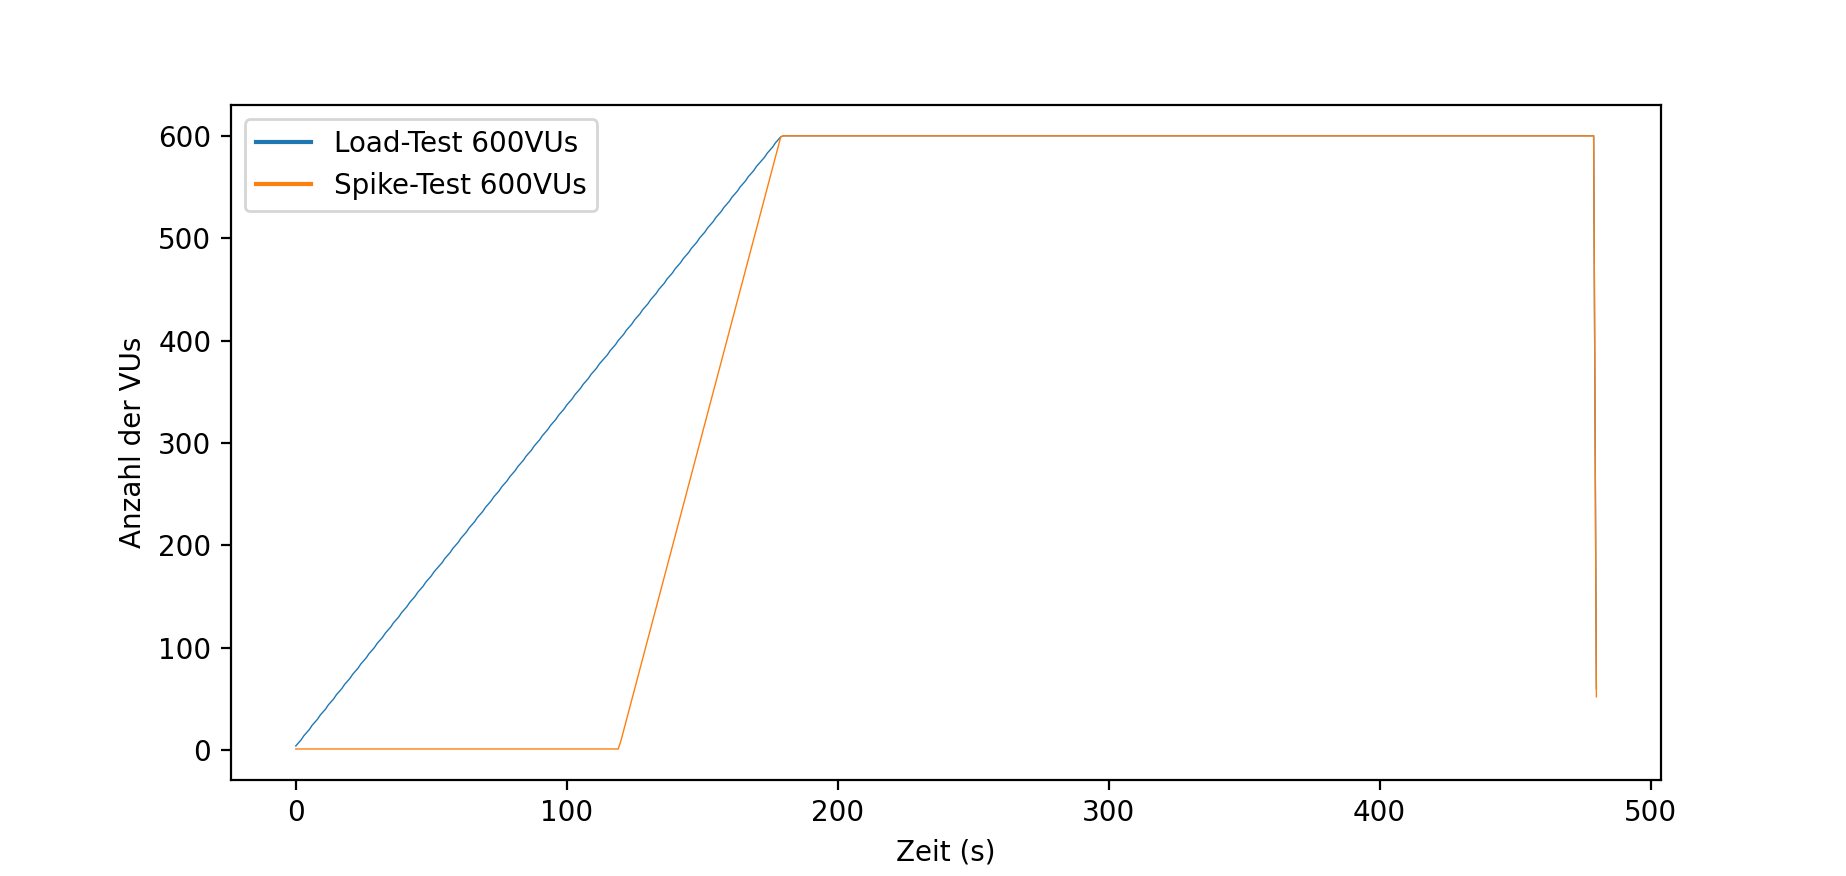
\includegraphics[width=\textwidth]{img/load600-vs-spike600.png}
    \caption[Load- und Spike-Test Vergleich]{Load- und Spike-Test Vergleich}
    \label{fig:load600-vs-spike600}
\end{figure}

Abbildung \ref{fig:load600-vs-spike600} zeigt die unterschiedlichen Test-Verläufe der beiden Tests. Die Anzahl der Benutzer steigt bei dem Load-Test von Anfang an kontinuierlich an und erreichen innerhalb von drei Minuten die maximale Grenze. Für den Spike-Test soll nach einer zwei-minütigen Warte-Phase, in der keine Benutzer auftreten, ein schneller Anstieg innerhalb von einer Minute auf die 600 Virtuelle Benutzer erfolgen. Der Anstieg des Spike-Tests ist also drei mal steiler als der des Load-Tests. 
Nach Erreichen der Obergrenze wird bei beiden Tests die Anzahl der Benutzer für fünf Minuten konstant gehalten. Dies lässt eventuelle Nachwirkungen des Skalierungsverhaltens der Lambda-Funktionen erkennen.


\subsubsection{Container}
Bei der Durchführung der Tests für den 128MB Container konnten keine Veränderungen der Performance für einen schnellen Anstieg der Benutzer gegenüber dem langsamen Anstieg festgestellt werden.

\subsubsection{Lambda}
Für die Lambda-Funktionen lassen sich keine eindeutigen Unterschiede in der Antwortzeit für die beiden verschiedenen Anstiegs-Intervalle feststellen. 


\begin{figure}[H]
    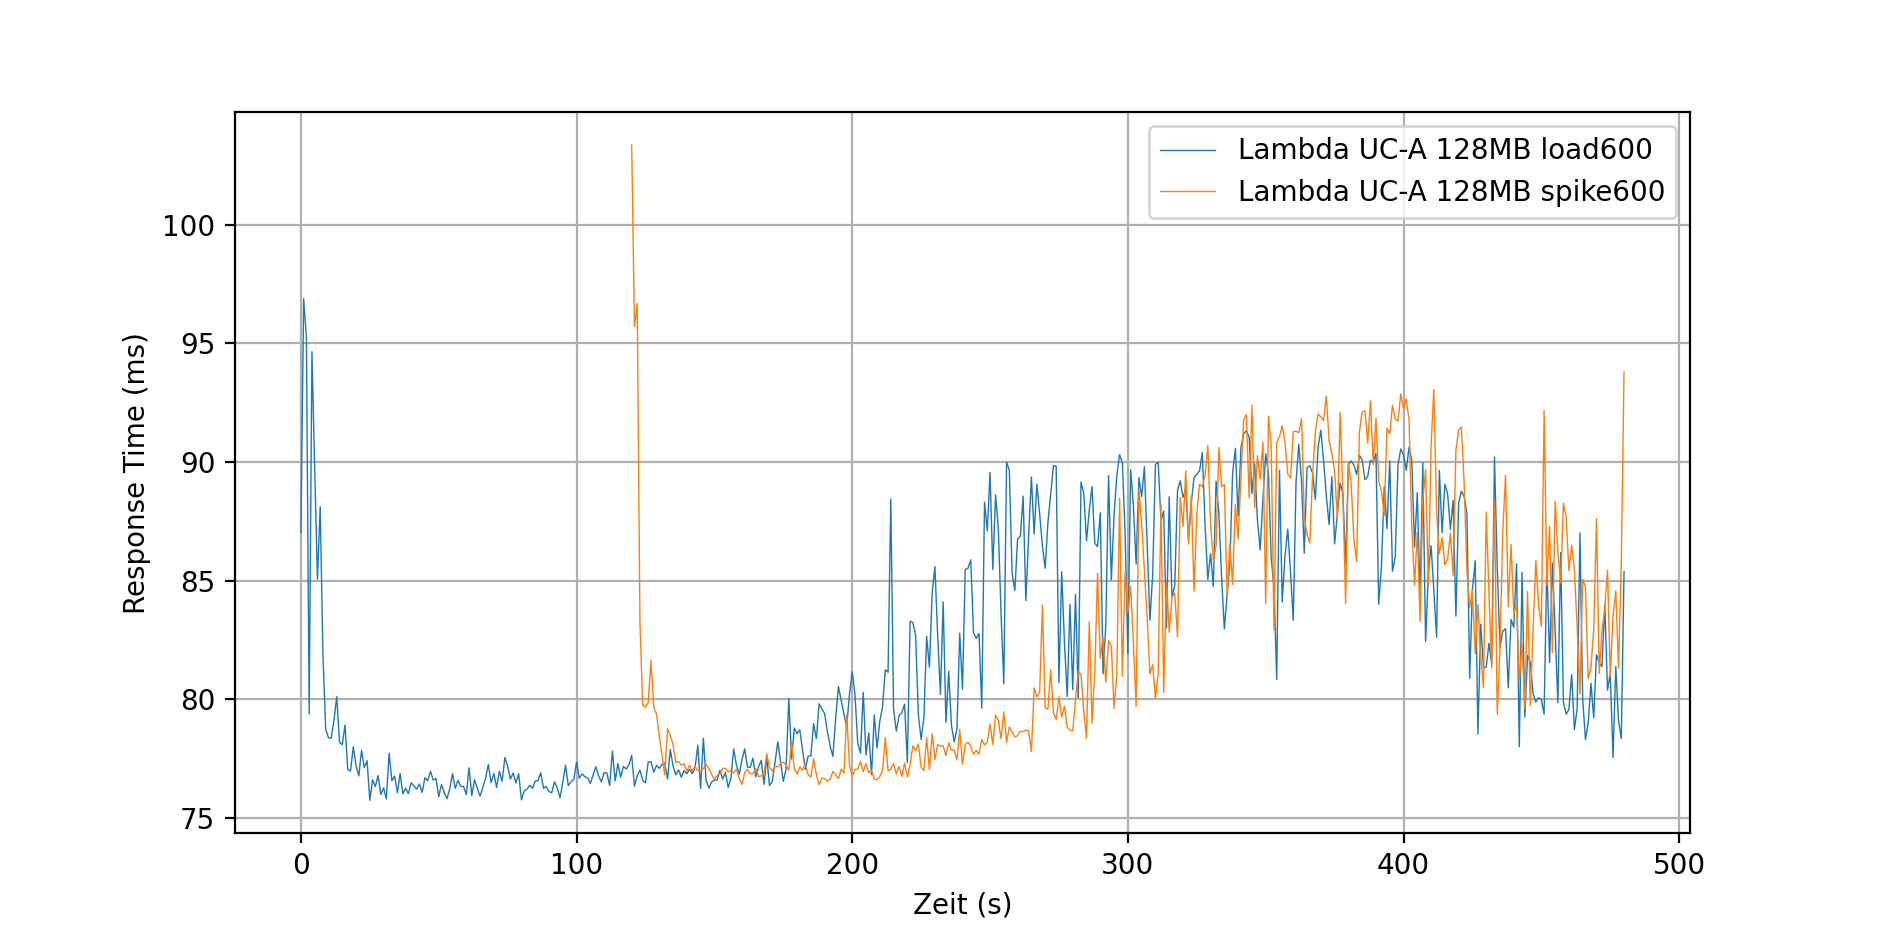
\includegraphics[width=\textwidth]{img/lambda-uca-load600-vs-spike600-example.png}
    \caption[Lambda Use-Case A Load- und Spike-Test Vergleich]{Lambda Use-Case A Load- und Spike-Test Vergleich}
    \label{fig:lambda-uca-load600-vs-spike600-example}
\end{figure}

Abbildung \ref{fig:lambda-uca-load600-vs-spike600-example} zeigt ein Vergleich der Load- und Stress-Tests für Use-Case A. Für den Load-Tests (blaue Linie) ist zu erkennen, dass sich nach anfänglich hohen Antwortzeiten von ca 95ms das Niveau bei 75ms - 80ms einpendelt. Ab 180 Sekunden (3 Minuten) ist die maximale User-Anzahl erreicht. Nach ca. 200 Sekunden überschreitet die Median-Antwortzeit für den Load-Test die 80ms Marke und erreicht ihren Höchststand nach ca. 350 Sekunden mit ca. 90ms. Danach sinkt die Median-Antwortzeit wieder trotz konstanter Nutzerzahlen.
Für den Spike-Test scheint es sich ähnlich zu verhalten. Auch wenn nach 180 Sekunden die 600 VUs erreicht wurden, klettert die Antwortzeit allerdings erst mehr als eine Minute später über die 80ms Marke. Der Spike-Test erreicht ebenso wie der Load-Test nach ca. 350 Sekunden sein Maximum; die Antwortzeit liegt mit ca. 93ms nur leicht über der des Load-Tests.

\begin{figure}[H]
    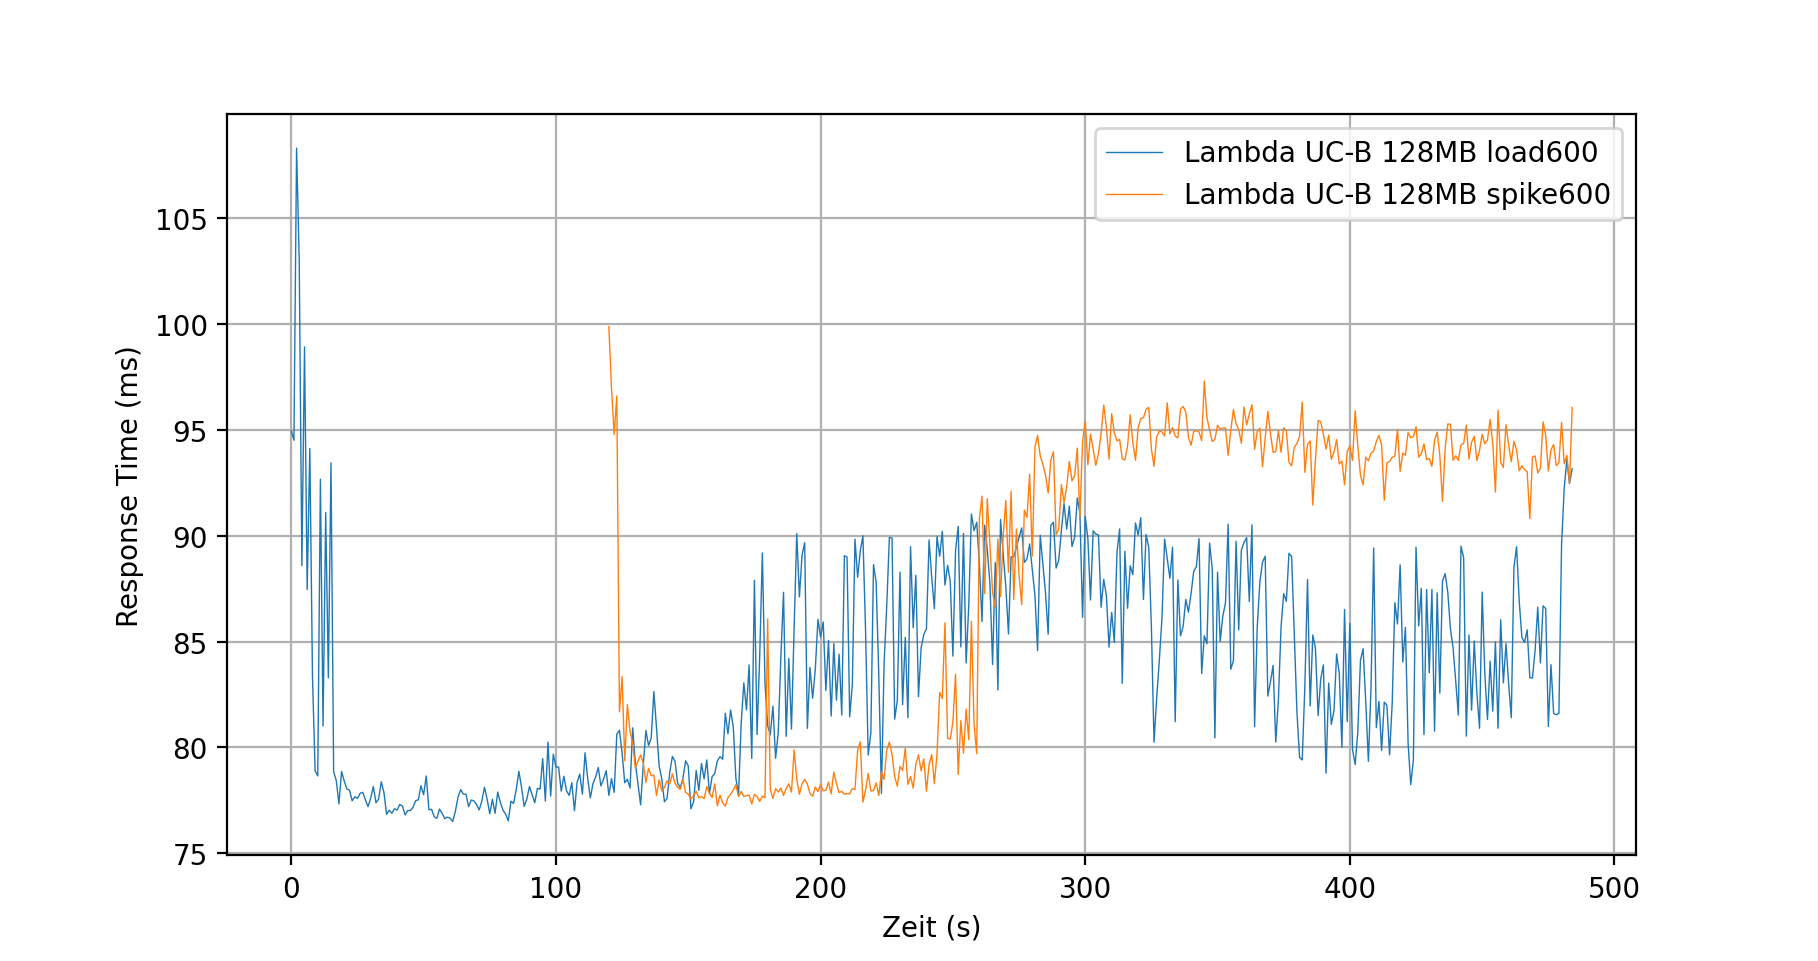
\includegraphics[width=\textwidth]{img/lambda-ucb-load600-vs-spike600-example.png}
    \caption[Lambda Use-Case B Load- und Spike-Test Vergleich]{Lambda Use-Case B Load- und Spike-Test Vergleich}
    \label{fig:lambda-ucb-load600-vs-spike600-example}
\end{figure}

Für Use-Case B (Abbildung \ref{fig:lambda-ucb-load600-vs-spike600-example}) sieht der Verlauf ähnlich aus, allerdings fällt die Kurve des Load-Tests nach Erreichen der höchsten Antwortzeit schneller ab als die des Spike-Test. Außerdem erreicht der Spike-Test mit ca. 95ms eine ca. 5ms höhere maximale Antwortzeit als der Load-Test. Interessant ist außerdem, dass die Antwortzeit des Load-Test eine größere Schwankung aufweist, als die des Spike-Tests, bei dem aufeinander folgende Werte stets relativ nah beieinander liegen.

Da die Antwortzeiten des Spike-Test trotz des dreimal schnelleren Anstiegs dennoch äußerst nah bei denen des Load-Tests liegen, lässt sich entgegen H1 annehmen, dass ein schneller Spike-Load kaum eine Veränderung der Antwortzeit mit sich bringt. Bei größeren Nutzerzahlen könnte dieser Effekt jedoch größer ausfallen.


\section{256MB Konfigurationen}
Als nächstes sollen Container und Lambda-Funktionen mit einer CPU- und Speicher-Größe von 256 Megabyte untersucht werden. Ziel dessen ist es, Unterschiede zu den in der vorangegangenen Sektion getesteten Konfigurationen zu erkennen.

\subsection{Pipe-Clean Tests}
Wie in Abbildung \ref{fig:pipe256-comparison} zu sehen ist, konnte keine Veränderung der Pipe-Clean Performance für die größere Variante festgestellt werden; weder für den Container noch für die Lambda-Funktionen.
\begin{figure}[H]
    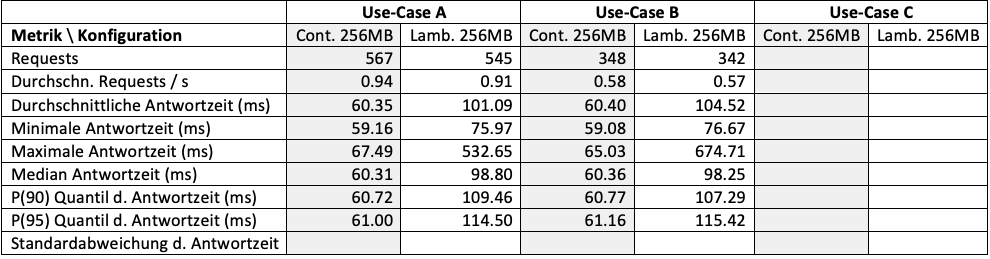
\includegraphics[width=\textwidth]{img/pipe256-comparison.png}
    \caption[Vergleich der Pipe-Clean Tests für 256MB]{Vergleich der Pipe-Clean Tests für 256MB}
    \label{fig:pipe256-comparison}
\end{figure}

\subsection{Stress-Tests}
Unter Annahme von H3 wird davon ausgegangen, dass der Container 256MB Speicher und CPU-Größe doppelt so viele Anfragen verarbeiten kann wie der Container mit 128MB. Da der kleinere Container bis zu 700 Benutzer bedienen konnte, wird im folgenden ein Stress-Test mit bis zu 1500 Benutzern durchgeführt, für den Fall dass er mehr als doppelt so viel verarbeiten kann.

Trotz des doppelt so großen Speichers und vCPUs konnte jedoch keine Verbesserung der maximalen Benutzer für die Container-Instanz erreicht werden. Genau wie der 128MB Container begann die Antwortzeit des 256MB Container bei ca. 700 VUs stark anzusteigen. Die Hypothese H3 kann also für diesen Fall nicht bestätigt werden.

Die Lambda-Tests wurden für diese Konfiguration nicht durchgeführt, da keine Verbesserung gegenüber der 128MB Variante zu vermutet wird.

\section{512MB Konfigurationen}
Als nächstes sollen Container und Lambda-Funktionen mit einer CPU- und Speicher-Größe von 512 Megabyte untersucht werden. 

\subsection{Pipe-Clean Tests}

\subsection{Stress-Tests}
Ein Stress-Test des Containers mit bis zu 1500 Benutzern, ergab für Use-Case A, dass die Antwortzeit des Containers ab einer VU-Anzahl von ca. 1400 Benutzern deutlich zunimmt. Mit Eintreten der 1400 Benutzer erreichte das Container Cluster ebenso eine CPU-Auslastung von 100 Prozent. Für Use-Case B musste ein weiterer Stress-Test durchgeführt werden, da bei 1500 Benutzern nur eine CPU-Auslastung von 58\% erreicht werden konnte. Der zweite Stress-Test wurde mit bis zu 2400 Benutzern durchgeführt. Bei ca. 2350 VUs wurde die maximale Auslastung des Containers erreicht.

Im Anschluss an die Stress-Tests des Containers wurden diese mit den gleichen Konfigurationen gegen die Lambda-Anwendung durchgeführt. 



\section{Skalierung und Optimierung}
\subsection{Container}
Da Container auf jedem Computer mit Unterstützung einer Container-Runtime laufen können, bieten sich vielfältige Wege an eine Container-Anwendung zu betreiben und zu skalieren. Deshalb kann in dieser Arbeit nicht auf alle eingegangen werden. Meist wird ein Container-Orchestrations-Tool verwendet, um das manuelle Verteilen der Container auf Computer-Clustern zu vermeiden. Bei Kubernetes gibt es den Horizontal Pod Autoscaler (HPA), der die automatische Skalierung von Pods in Abhängigkeit der CPU-Auslastung ermöglicht\cite{noauthor_horizontal_nodate-1}. Auch bei Nutzung des AWS Elastic Kubernetes Service (EKS) ist ein automatische Skalierung möglich\cite{noauthor_horizontal_nodate}. Auch die Nutzung eines Vertical Pod Autoscaler (VPA) ist möglich, der automatisch die Ressourcen einzelner Container skaliert\cite{noauthor_vertical_nodate}. Es kann auch ein Cluster Autoscaler verwendet werden, um zusätzlich zu der Anzahl der Container auch die Anzahl der Kubernetes-Knoten hoch zu skalieren\cite{noauthor_cluster_nodate}.
Auf die Performance-Tests all dieser Konfigurationen kann in dieser Arbeit unmöglich eingegangen werden, da es zu diesem Thema zu viele Möglichkeiten und auch Wege zur Optimierung gibt. Beispielsweise lässt sich die Schwelle der CPU-Auslastung einstellen, ab der die Anzahl der Container hoch- oder runter-skaliert werden soll. Liegt die Schwelle zu niedrig, skaliert das System evtl. zu früh und die Kosten steigen. Liegt die Schwelle zu hoch, skaliert das System evtl. zu spät und die Performanz sinkt.

In dieser Arbeit wurde AWS ECS mit dem Fargate-Starttyp verwendet, um die Einstellung eines Clusters nicht vornehmen zu müssen. Fargate verwaltet die Knoten des Clusters automatisch. Der ordinäre Weg der Cluster-Erstellung wäre es, mehrere Virtuelle Maschinen zu starten, zu konfigurieren und jede dem Cluster zuzuweisen. Durch die Nutzung von Fargate kann die Konfiguration von Container-Clustern also erheblich vereinfacht werden. ECS und Fargate bieten mit Auto-Scaling auch eine Möglichkeit der automatischen Skalierung an. Diese funktioniert zusammen mit AWS CloudWatch Alarmen. Dazu lässt sich eine von zwei verschiedenen Policies einstellen.

Bei einer Step Scaling Policy lassen sich, ähnlich wie bei Kubernetes HPA, Grenzen für die Skalierung auf Basis von CloudWatch Metriken, also bspw. CPU- oder Arbeitsspeicher-Auslastung, festlegen. CloudWatch überprüft dann in bestimmten Intervallen die Metriken und schlägt Alarm, wenn eine Metrik über oder unter dem spezifizierten Schwellwert liegt. Fargate reagiert auf den Alarm und skaliert die Anzahl der Container innerhalb des Clusters hoch oder herunter. 

Bei einer Target Tracking Policy, lässt sich für Metriken ein Ziel festlegen, das eingehalten werden soll. Beispielweise könnte man ein Ziel von 75\% CPU-Auslastung festlegen. Mithilfe der CloudWatch Alarme wird dann versucht, dieses Ziel möglichst einzuhalten. 

Problematisch ist allerdings die Größe des Intervalls, in dem die Metriken überprüft werden können. Standardmäßig kann dies nur alle fünf Minuten erfolgen. Träfe die Container-Anwendung eine plötzliche Spitzenlast, würde es fünf Minuten dauern, bis reagiert und die Kapazität erhöht werden könnte. Nach Absprache mit AWS kann sich dieses Intervall auf eine Minute senken lassen. Dies ist allerdings, verglichen mit den Skalierungsmöglichkeiten von AWS Lambda, noch immer zu langsam für Anwendungen die hochverfügbar sein müssen.

Wichtig für eine schnelle Skalierung ist vor allem auch die Größe des Containers. Da bei jeder neu hinzugefügten Container-Instanz das Container-Image von der Registry heruntergeladen werden muss, ist es notwendig, die Image-Größe möglichst zu minimieren. Zum Einsatz kommende Techniken sind hierbei beispielsweise die Nutzung eines Alpine-Images als Basis-Image, einer besonders kleinen Linux-Distribution, Multi-Stage Builds, mit denen unnötige Dateien entfernt werden können oder Layer-Merging, bei dem die Anzahl der Docker-Layer minimiert wird.


\subsection{Lambda}
Lambda ist ein von Natur aus horizontal skalierendes System, daher müssen vom Entwickler theoretisch keine Einstellungen vorgenommen werden, um eine hochverfügbare Anwendung zu schaffen. Um auch Cold-Starts möglichst zu vermeiden, lässt sich die gewollte Nebenläufigkeit allerdings auch schon vor einem Benutzer-Ansturm definieren (Provisioned Concurrency). Lambda startet dann bereits Funktionen vor, die dann bei Bedarf keinen Kaltstart mehr erfordern, sondern direkt einen Warmstart durchführen können. Kombinieren lässt sich dies mit Autoscaling, um die provisionierte Kapazität an steigende Anfragezahlen anzupassen. 

Auch die Größe des Arbeitsspeicher einer Lambda-Funktion kann einen Einfluss auf das Skalierungsverhalten nehmen. Da eine Funktion mit größerem Speicher auch mehr CPU zugewiesen bekommt, können Anfragen, bei besonders CPU-intensiven Aufgaben, schneller verarbeitet werden und es werden eventuell weniger nebenläufige Funktionen und damit weniger Cold-Starts benötigt. Es gibt Tools wie "`AWS Lambda Power Tuning"'\cite{casalboni_alexcasalboniaws-lambda-power-tuning_2021}, die es für solche Funktionen ermöglichen, die beste Konfiguration zu finden.

Es gibt darüber hinaus vielfältige Wege, die Coldstart Zeit einer Lambda-Funktion zu verringern. Ähnlich zum Docker-Container, hat auch die Größe einer Lambda-Funktion Einfluss auf die Startzeit. Denn bei jedem Coldstart muss der Funktions-Code in den Lambda-Container geladen werden. Bei einigen Sprachen wie Java oder .NET macht ebenfalls die Konfiguration des Lambda-Arbeitsspeichers einen großen Unterschied\cite{malishev_aws_2019}. 

Lambda ist also auch nicht ohne weiteres eine Blaupause für jede beliebige Anwendung. Es lässt sich für jede Funktion eine vor-provisionierte Concurrency, Autoscaling und die Größe der Funktion einstellen. 

\section{Kosten}

\subsection{Container}
Wie schon in der vorherigen Sektion erwähnt gibt es viele verschiedene Wege, Container-Anwendungen in der Public Cloud zu betreiben. Für die Kosten-Schätzung werden deshalb nur der Betrieb der Anwendung mit AWS ECS Fargate-Starttyp und Amazon Elastic Kubernetes Service betrachtet.

Bei Fargate wird die Abrechnung in die gewählte Arbeitsspeicher und vCPU-Größe unterteilt. Der Preis für ein Arbeitsspeicher Gigabyte pro Stunde beträgt aktuell 0,00511\$ und der pro vCPU pro Stunde 0,04656\$.  \\


\begin{equation}
Kosten = Tasks * Stunden * Tage * (SpeicherGB * 0,00511\$ + AnzahlvCPUs * 0,04656\$)
\end{equation}

Es wird davon ausgegangen, dass mindestens ein Task dauerhaft laufen muss, damit der Service erreichbar bleibt. Für die in dieser Arbeit verwendete 128MB und 256MB Konfigurationen (mit 0.25 vCPU) ergäben sich für einen laufenden Task pro Monat (30 Tage) und Dauerbetrieb (24 Stunden pro Tag) Kosten von: \\

$Kosten = 1 * 24 * 30 * (0,5 * 0,00511\$ + 0,25 * 0,04656\$) = 10,22\$$ \\
(Stimmt tatsächlich mit den abgerechneten Kosten überein: 0,34\$ * 24 Tage = 10,22\$)

Die folgende Übersicht zeigt die monatlichen Kosten einer Instanz für die unterschiedlichen in dieser Arbeit verwendeten Konfigurations-Größen:

\begin{itemize}
    \item 128MB = 0,5GB und 0,25 vCPU = 10,22\$
    \item 256MB = 0,5GB und 0,25 vCPU = 10,22\$
    \item 512MB = 1  GB und 0,5  vCPU = 20,44\$
    \item 1024MB = 2 GB und 1    vCPU = 40,88\$
\end{itemize}
Für eine n-fache Anzahl an Tasks ergeben sich auch die n-fachen Kosten pro Monat. Variationen in den Anzahlen der Tasks aufgrund von (Auto-)Skalierung lassen sich nicht voraussagen und daher nicht berechnen.


\subsection{Lambda}
Die Ausführung von Lambda-Funktionen wird nach der Ausführungszeit in Millisekunden abgerechnet. Dabei zählt die Zeit eines Cold-Starts mit in die Berechnung ein. Auch die konfigurierte Arbeitsspeichergröße fließt mit in das Ergebnis ein. Derzeit berechnet AWS in der Region Frankfurt (eu-central-1) Kosten von 0,0000166667 US-Dollar pro GB-Sekunde\cite{noauthor_lambda_nodate}. Zusätzlich müssen pro 1.000.000 Ausführungen im Monat noch einmal 0,20 US-Dollar Anforderungsgebühren gezahlt werden. AWS bietet ein kostenloses Nutzenkontingent von 400.000 Aufrufen pro Funktion im Monat an.

Für die Ausführung der Lambda-Funktionen wird ein Event-Auslöser für REST-Anfragen benötigt. Dazu wurde in dieser Arbeit Amazon API Gateway verwendet, welches eingehende Requests auf die vorgesehene Lambda-Funktion weiterleitet. Für die Nutzung des API Gateways fallen extra Kosten an. Bei Nutzung des Serverless Frameworks wird automatisch eine API des Typs REST erstellt. Es fallen für die Verwendung dieses API-Typs Kosten von 3,70 Euro pro einer Millionen Aufruf an. Diese werden für jede API gezählt und gelten damit nicht für jede einzelne aufgerufene Lambda-Funktion. Es gibt Vergünstigungen ab 333 Millionen Aufrufen im Monat. Zuzügliche Preise für Caching werden hierbei nicht einberechnet. AWS bietet für das API Gateway ebenso ein kostenloses Nutzenkontingent von einer Millionen Aufrufen im Monat\cite{noauthor_amazon_nodate}.

\begin{equation}
\begin{split}
Kosten = Aufrufe * \frac{MedianMs}{1000ms} * \frac{FunktionsMb}{1024Mb} * 0,0000166667\$ \\
+ \frac{Aufrufe}{1.000.000} * (0,20\$ + 3,70\$)
\end{split}
\end{equation}

Der Preis für eine Millionen Aufrufe einer einzigen Lambda-Funktion mit einer Größe von 128MB und einer medianen Laufzeit von 70ms ergibt (die kostenlosen Nutzenkontingente nicht mit einberechnet): \\

Datenverarbeitungs-Sekunden = 1.000.000 * 70ms / 1000ms = 70.000s   \\
Datenverarbeitung GB-s = 70.000 * 128 MB / 1024 = 8.750 GB-s    \\
Kosten Lambda = 8.750 GB-s * 0,0000166667 + 0,20\$ Anforderungsgebühren = 0,35 \$     \\

Hinzu kommen die Kosten von 3,70\$ für API Gateway. Die Gesamtkosten betrügen damit 4,05\$ für eine Millionen Aufrufe dieser Funktion im Monat.    \\

Die folgende Übersicht zeigt die Kosten pro 1.000.000 Aufrufe für die unterschiedlichen Funktions-Größen:
\begin{itemize}
    \item 128MB = 4,05\$
    \item 256MB = 4,19\$
    \item 512MB = 4,48\$
    \item 1024M = 5,07\$
\end{itemize}

Da bei Lambda im  Gegensatz zu ECS/Fargate nur die tatsächlich aktive Zeit der Funktion berechnet wird, lässt sich grob abschätzen, wie viele Funktionsaufrufe zu dem gleichen Preis der Fargate Nutzung von einem Container möglich sind (siehe vorherige Sektion). Die Umstellung der Formel ergibt:

\begin{equation}
Aufrufe = \frac{Kosten}{\frac{MedianMs}{1000ms} * \frac{FunktionsMb}{1024Mb} * 0,0000166667\$ + \frac{0,20\$ + 3,70\$}{1.000.000}}
\end{equation}

Ausgehend von den Kosten der Container Varianten und einer Medianen Antwortzeit von 70ms ergeben sich folgende Werte: 

\begin{itemize}
    \item 128MB (10,22\$): 2.526.055 Aufrufe
    \item 256MB (10,22\$): 2.438.170 Aufrufe
    \item 512MB (20,44\$): 4.559.106 Aufrufe
    \item 1024MB (40,88\$): 8.068.417 Aufrufe
\end{itemize}